\documentclass[border=2pt]{standalone}

% Drawing
\usepackage{tikz}

% Notation
\usepackage{amsmath}

\begin{document}
	
	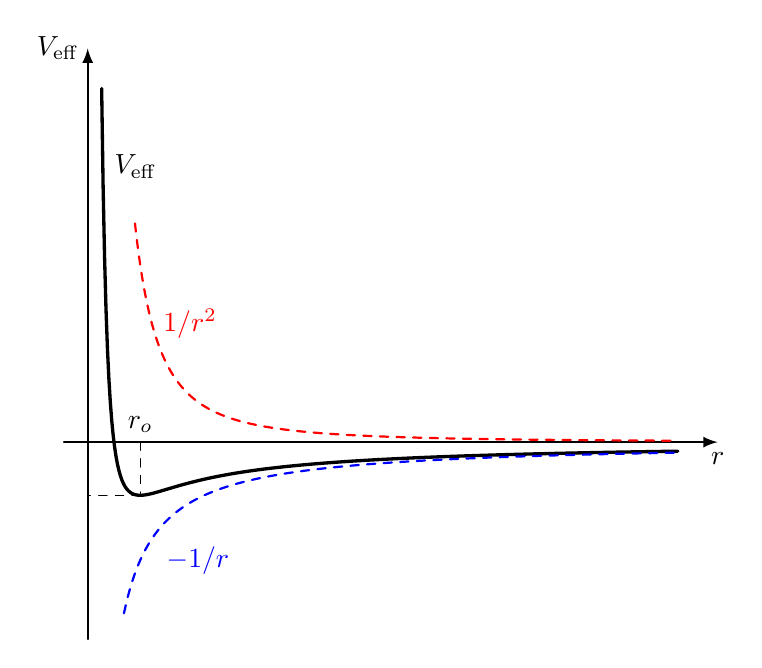
\begin{tikzpicture}[line cap=round]
%		%Grid
%		\draw[thin, dotted] (0,0) grid (8,8);
%		\foreach \i in {1,...,8}
%		{
%			\node at (\i,-2ex) {\i};	
%		}
%		\foreach \i in {1,...,8}
%		{
%			\node at (-2ex,\i) {\i};	
%		}
%		\node at (-2ex,-2ex) {0};
		
		% Axis
		\draw[thick, -latex] (-2ex,0) -- (8,0) node[below] {$r$};
		\draw[thick, -latex] (0,-2.5) -- (0,5) node[left] {$V_\text{eff}$};	
		
		% Plot Function
		\draw[domain=0.177:7.5, samples=400, variable=\r, very thick] plot ({\r},{0.3/(\r*\r)-0.9/\r});
		\draw[domain=0.6:7.5, samples=300, variable=\r, thick, dashed, red] plot ({\r},{1/(\r*\r)});
		\draw[domain=0.46:7.5, samples=300, variable=\r, thick, dashed, blue] plot ({\r},{-1/(\r)});
		
		% Dashed
		\draw[dashed] (2/3,0) -- +(0,-0.65) node[pos=0, above] {$r_o$};
		\draw[dashed] (2/3,-0.68) -- (0,-0.68);		
		
		% Nodes
		\node at (0.6,3.5) {$V_\text{eff}$};
		\node[red] at (1.3,1.5) {$1/r^2$};
		\node[blue] at (1.4,-1.5) {$-1/r$};
	\end{tikzpicture}
	
\end{document}
